\documentclass[a4paper, 12pt]{letter}
\usepackage[utf8]{inputenc}
\usepackage[scaled]{helvet}
\renewcommand\familydefault{\sfdefault}
\usepackage[T1]{fontenc}
\usepackage[francais]{babel}
\usepackage[left=2.5cm,top=6cm,right=2.5cm,bottom=2.5cm]{geometry}
\usepackage{graphicx}
\begin{document}
\pagenumbering{gobble} %no page number

% ---------------- Le contenu commence ici ----------------
\hbox to \textwidth{\hfill
	\vbox{
		\hbox{<title>}
		\hbox{<firstName> <lastName>}
		\hbox{<livesAt>}
		\hbox{<street> <numStreet>}
		\hbox{<postCode> <locality>}
		\bigbreak
		\bigbreak
		\bigbreak
		\hbox{Veyrier, le <sendDate> / <initials>}
	}
}

\bigbreak

\begin{flushleft}
	\textbf{Mise en suspens de votre dossier de candidature}
	\line(1,0){455}
\end{flushleft}
\bigbreak

<title>,

Nous accusons réception de votre candidature spontanée du <requestDate> qui a retenu toute notre attention.

Néanmoins, compte tenu des éléments positifs de votre parcours et sauf avis contraire de votre part, nous souhaitons conserver votre dossier si toutefois un poste correspondant à votre profil venait à se libérer.

Aussi, nous vous encourageons à déposer votre candidature en ligne sur le site de l’AGEMS (Association Genevoise des établissements médico-sociaux).

En vous remerciant de l’intérêt que vous portez à l’EMS Les Châtaigniers, nous vous prions d’agréer, <title>, nos salutations distinguées.

\bigbreak
\bigbreak
\bigbreak
\bigbreak

\hbox to \textwidth{\hfill
	\vbox{
		\hbox{EMS Les Châtaigniers}
	}
}
\begin{flushright}
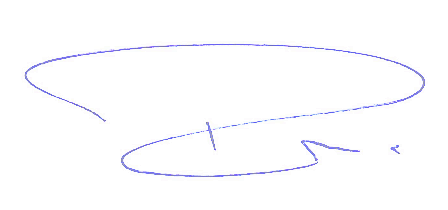
\includegraphics{sign.png}
\end{flushright}

\hbox to \textwidth{\hfill
	\vbox{
		\hbox{Samuel Moix, Directeur adjoint}
	}
}

\bigbreak
\bigbreak

<folder>

\end{document}
